\section{Experiments}
\label{sec:experiments}

We organize the experiments around three questions: whether the regime-local specialists support autonomous prediction, whether
physical-space fusion improves prediction near regime transitions, and how the main local architectural choices affect prediction.
The three incompressible-flow benchmarks play complementary roles in answering these questions. All are two-dimensional systems in which varying the Reynolds number traverses steady, Hopf-onset, and periodic regimes. The circular-cylinder benchmark provides the local architecture ablation, the centered-square benchmark evaluates cross-regime routing and fusion in the $S$--$H$ and $H$--$P$ overlaps, and the fluidic-pinball benchmark provides the autonomous comparison with a classical POD--Galerkin ROM. Table~\ref{tab:benchmark_summary} summarizes the benchmark scope and roles. All splits are made at the level of complete parameter trajectories rather than individual snapshots or rollout windows; chart-wise parameter ranges and split counts are reported in Appendix~\ref{app:implementation}.

We report relative physical-field errors $E_u$ and $E_p$ in percent; their weighted definitions and benchmark-specific aggregation rules are given in Appendix~\ref{app:implementation}. For routing and fusion comparisons, $E_{\mathrm{joint}}=E_u+E_p$. The sum of displayed component errors can differ slightly from the reported joint error because values are rounded independently. A rollout window is labeled ``Divergent'' if it violates the predefined rollout-divergence criterion, either through a non-finite state or a
threshold violation. N/E denotes a setting that is not evaluable under this criterion; table-specific notes identify the cause.

\begin{table}[t]
\centering
\caption{
Experimental scope and benchmark roles.
Local rank pairs $(r_u,r_p)$ and rollout horizons $K$ are ordered
$S,H,P$.
Additional overlap and periodic-core settings are specified in their
respective comparisons.
}
\label{tab:benchmark_summary}
\small
\setlength{\tabcolsep}{4pt}
\begin{tabular}{@{}>{\raggedright\arraybackslash}p{2.15cm}
>{\raggedright\arraybackslash}p{1.30cm}
>{\raggedright\arraybackslash}p{4.05cm}
>{\raggedright\arraybackslash}p{1.80cm}
>{\raggedright\arraybackslash}p{2.50cm}@{}}
\toprule
Benchmark & $Re$ range & Local ranks ($S,H,P$) & Rollout horizons & Primary role \\
\midrule
Circular cylinder
& 20--200
& $(32,32),\ (32,32),\ (32,32)$
& $56/56/48$
& Local architecture ablation \\
\addlinespace
Centered square
& 50--150
& $(5,4),\ (11,11),\ (28,26)$
& $16/48/24$
& Cross-regime routing/fusion \\
\addlinespace
Fluidic pinball
& 10--60
& $(4,3),\ (5,5),\ (17,16)$
& $56/56/32$
& Autonomous ROM baseline \\
\bottomrule
\end{tabular}
\end{table}



\subsection{Do local specialists support accurate autonomous rollouts?}

We first examine whether the regime-local specialists maintain accurate predictions under autonomous rollout on the fluidic-pinball benchmark. Table~\ref{tab:pinball_autonomous} compares the learned specialists with a classical POD--Galerkin ROM over the Steady, Hopf, and Periodic regimes.

RAL-MoE-ROM achieves low physical-field errors across all four evaluation settings. In the Hopf and Periodic settings where POD--Galerkin errors are reported, the learned specialists consistently reduce both velocity and pressure
errors, with the largest differences appearing in pressure. For example, the Hopf joint error decreases from $48.94\%$ to $2.085\%$, while the standard Periodic error decreases from $43.20\%$ to $0.8415\%$. The longer-horizon Periodic-core evaluation shows the same trend, with $E_{\mathrm{joint}}$ reduced from $41.91\%$ to $1.672\%$. Together, these results show that the learned specialists maintain low physical-field error over the evaluated autonomous horizons.

\begin{table}[htbp]
\centering
\caption{
Autonomous local-specialist prediction on the fluidic-pinball benchmark. Errors are physical-field percentages; lower is better. Periodic core denotes the longer-horizon periodic evaluation; complete protocol details are given in Appendix~\ref{app:pinball}. A dash indicates that no baseline error is reported.
}
\label{tab:pinball_autonomous}
\small
\setlength{\tabcolsep}{5pt}
\begin{tabular}{@{}llrrr@{}}
\toprule
Evaluation setting & Model & $E_u$ & $E_p$ & $E_{\mathrm{joint}}$ \\
\midrule
Steady ($K=56$)
& POD--Galerkin
& -- & -- & -- \\
& RAL-MoE-ROM
& 0.2247 & 0.7593 & 0.9840 \\
\addlinespace

Hopf ($K=56$)
& POD--Galerkin
& 0.4378 & 48.50 & 48.94 \\
& RAL-MoE-ROM
& 0.0995 & 1.986 & 2.085 \\
\addlinespace

Periodic ($K=32$)
& POD--Galerkin
& 1.641 & 41.56 & 43.20 \\
& RAL-MoE-ROM
& 0.2897 & 0.5518 & 0.8415 \\
\addlinespace

Periodic core ($K=56$)
& POD--Galerkin
& 2.555 & 39.36 & 41.91 \\
& RAL-MoE-ROM
& 0.6222 & 1.050 & 1.672 \\
\bottomrule
\end{tabular}
\end{table}

A complementary POD--DeepONet experiment further separates one-step prediction from autonomous rollout.
The model attains $E_u=1.5921\%$ and $E_p=23.3447\%$ on 4,228 held-out one-step pairs, but only one of 28 held-out trajectories completes the prescribed autonomous rollout evaluation. Because its temporal cadence differs from that of the Periodic specialist, we use this result only to contrast one-step prediction with autonomous rollout, rather than as a matched long-horizon accuracy comparison (Appendix~\ref{app:pinball}).





\subsection{Does physical-space fusion improve prediction in regime overlaps?}
To evaluate the second routing level while holding the local specialists fixed, we compare the centered-square $S$--$H$ and $H$--$P$ overlaps at $K=24$ (Table~\ref{tab:routing_fusion}). We compare hard E2 Top-1 routing with two simple fusion rules (equal weighting and E2-probability weighting) and the learned T2-C gate; a diagnostic convex oracle provides an a posteriori reference. To test whether T2-C benefits specifically from physical-history information, we additionally include an architecture-matched T2-C $\mu$-only ablation. The same gate architecture and optimization protocol are retained, but the standardized history-descriptor channels are set to zero. This preserves the gate parameterization and trainable parameter count while removing history information.


The $\mu$-only ablation reveals that parameter conditioning alone has overlap-dependent value. For $S$--$H$, its joint error is essentially unchanged relative to E2-probability blending ($2.1846\%$ versus $2.1847\%$), whereas for $H$--$P$ it improves the same baseline from $1.6618\%$ to $1.1504\%$. Adding the physical-history descriptor improves both overlaps further, reducing $E_{\mathrm{joint}}$ to $1.1958\%$ and $0.8465\%$, respectively. Relative to the a posteriori best fixed-specialist reference, full T2-C reduces joint error by $30.9\%$ on $S$--$H$ and $29.9\%$ on $H$--$P$. Relative to the deployable E2 Top-1 router, the corresponding reductions are $30.9\%$ and $54.2\%$. The fixed-run T2-C errors are also close to the diagnostic convex oracle in both overlaps. Representative reconstructed fields and velocity-error maps are shown in Figure~\ref{fig:square_overlap}.

Across three paired gate-training seeds, full T2-C outperforms the architecture-matched $\mu$-only gate in every run for both overlaps.
Across the three paired runs, the mean reduction relative to $\mu$-only is $45.3\%$ for $S$--$H$ and $26.2\%$ for $H$--$P$. Full T2-C yields
$E_{\mathrm{joint}}=1.1957\pm0.0001\%$ on $S$--$H$ and $0.8500\pm0.0035\%$ on $H$--$P$, where $\pm$ denotes the sample standard
deviation across the three gate-training seeds. Only gate training is repeated across seeds; the specialists, E2 router, candidate rollouts, data partitions, normalization, and optimization protocol are fixed. These statistics therefore characterize gate-training variability rather than full-pipeline uncertainty. Component-wise errors and seed-level results are reported in Appendix~\ref{app:square}, with the corresponding fluidic-pinball overlap study in Appendix~\ref{app:pinball}.


\begin{table}[t]
\centering
\caption{
Fixed-run cross-regime routing and fusion on the centered-square benchmark at $K=24$. Entries are terminal-step $E_{\mathrm{joint}}$ (\%); lower is better. T2-C $\mu$-only uses the same gate architecture with all standardized history-descriptor channels set to zero. The oracle is an a posteriori convex reference and is not available at inference. Three-seed gate-training variability is reported separately in
Appendix~\ref{app:square}. Bold marks the best deployable method in this fixed-run comparison.
}
\label{tab:routing_fusion}
\small
\setlength{\tabcolsep}{3.5pt}
\begin{threeparttable}
\begin{tabular}{@{}lrrrrrrr@{}}
\toprule
Overlap & Best fixed$^\ast$ & E2 Top-1 & Equal & E2 prob. blend & T2-C $\mu$-only & T2-C & Oracle\\
\midrule
$S$--$H$ & 1.7298 & 1.7298 & 3.0321 & 2.1847 & 2.1846 & \textbf{1.1958} & 1.1842 \\
$H$--$P$ & 1.2079 & 1.8473 & 1.6146 & 1.6618 & 1.1504 & \textbf{0.8465} & 0.8384 \\
\bottomrule
\end{tabular}
\begin{tablenotes}[flushleft]
\footnotesize
\item[$\ast$] Best fixed denotes the a posteriori fixed-specialist reference selected by aggregate evaluation error over the corresponding overlap (Hopf for $S$--$H$, Periodic for $H$--$P$). It is not a routing strategy available at inference.
\end{tablenotes}
\end{threeparttable}
\end{table}

\begin{figure}[t]
\centering
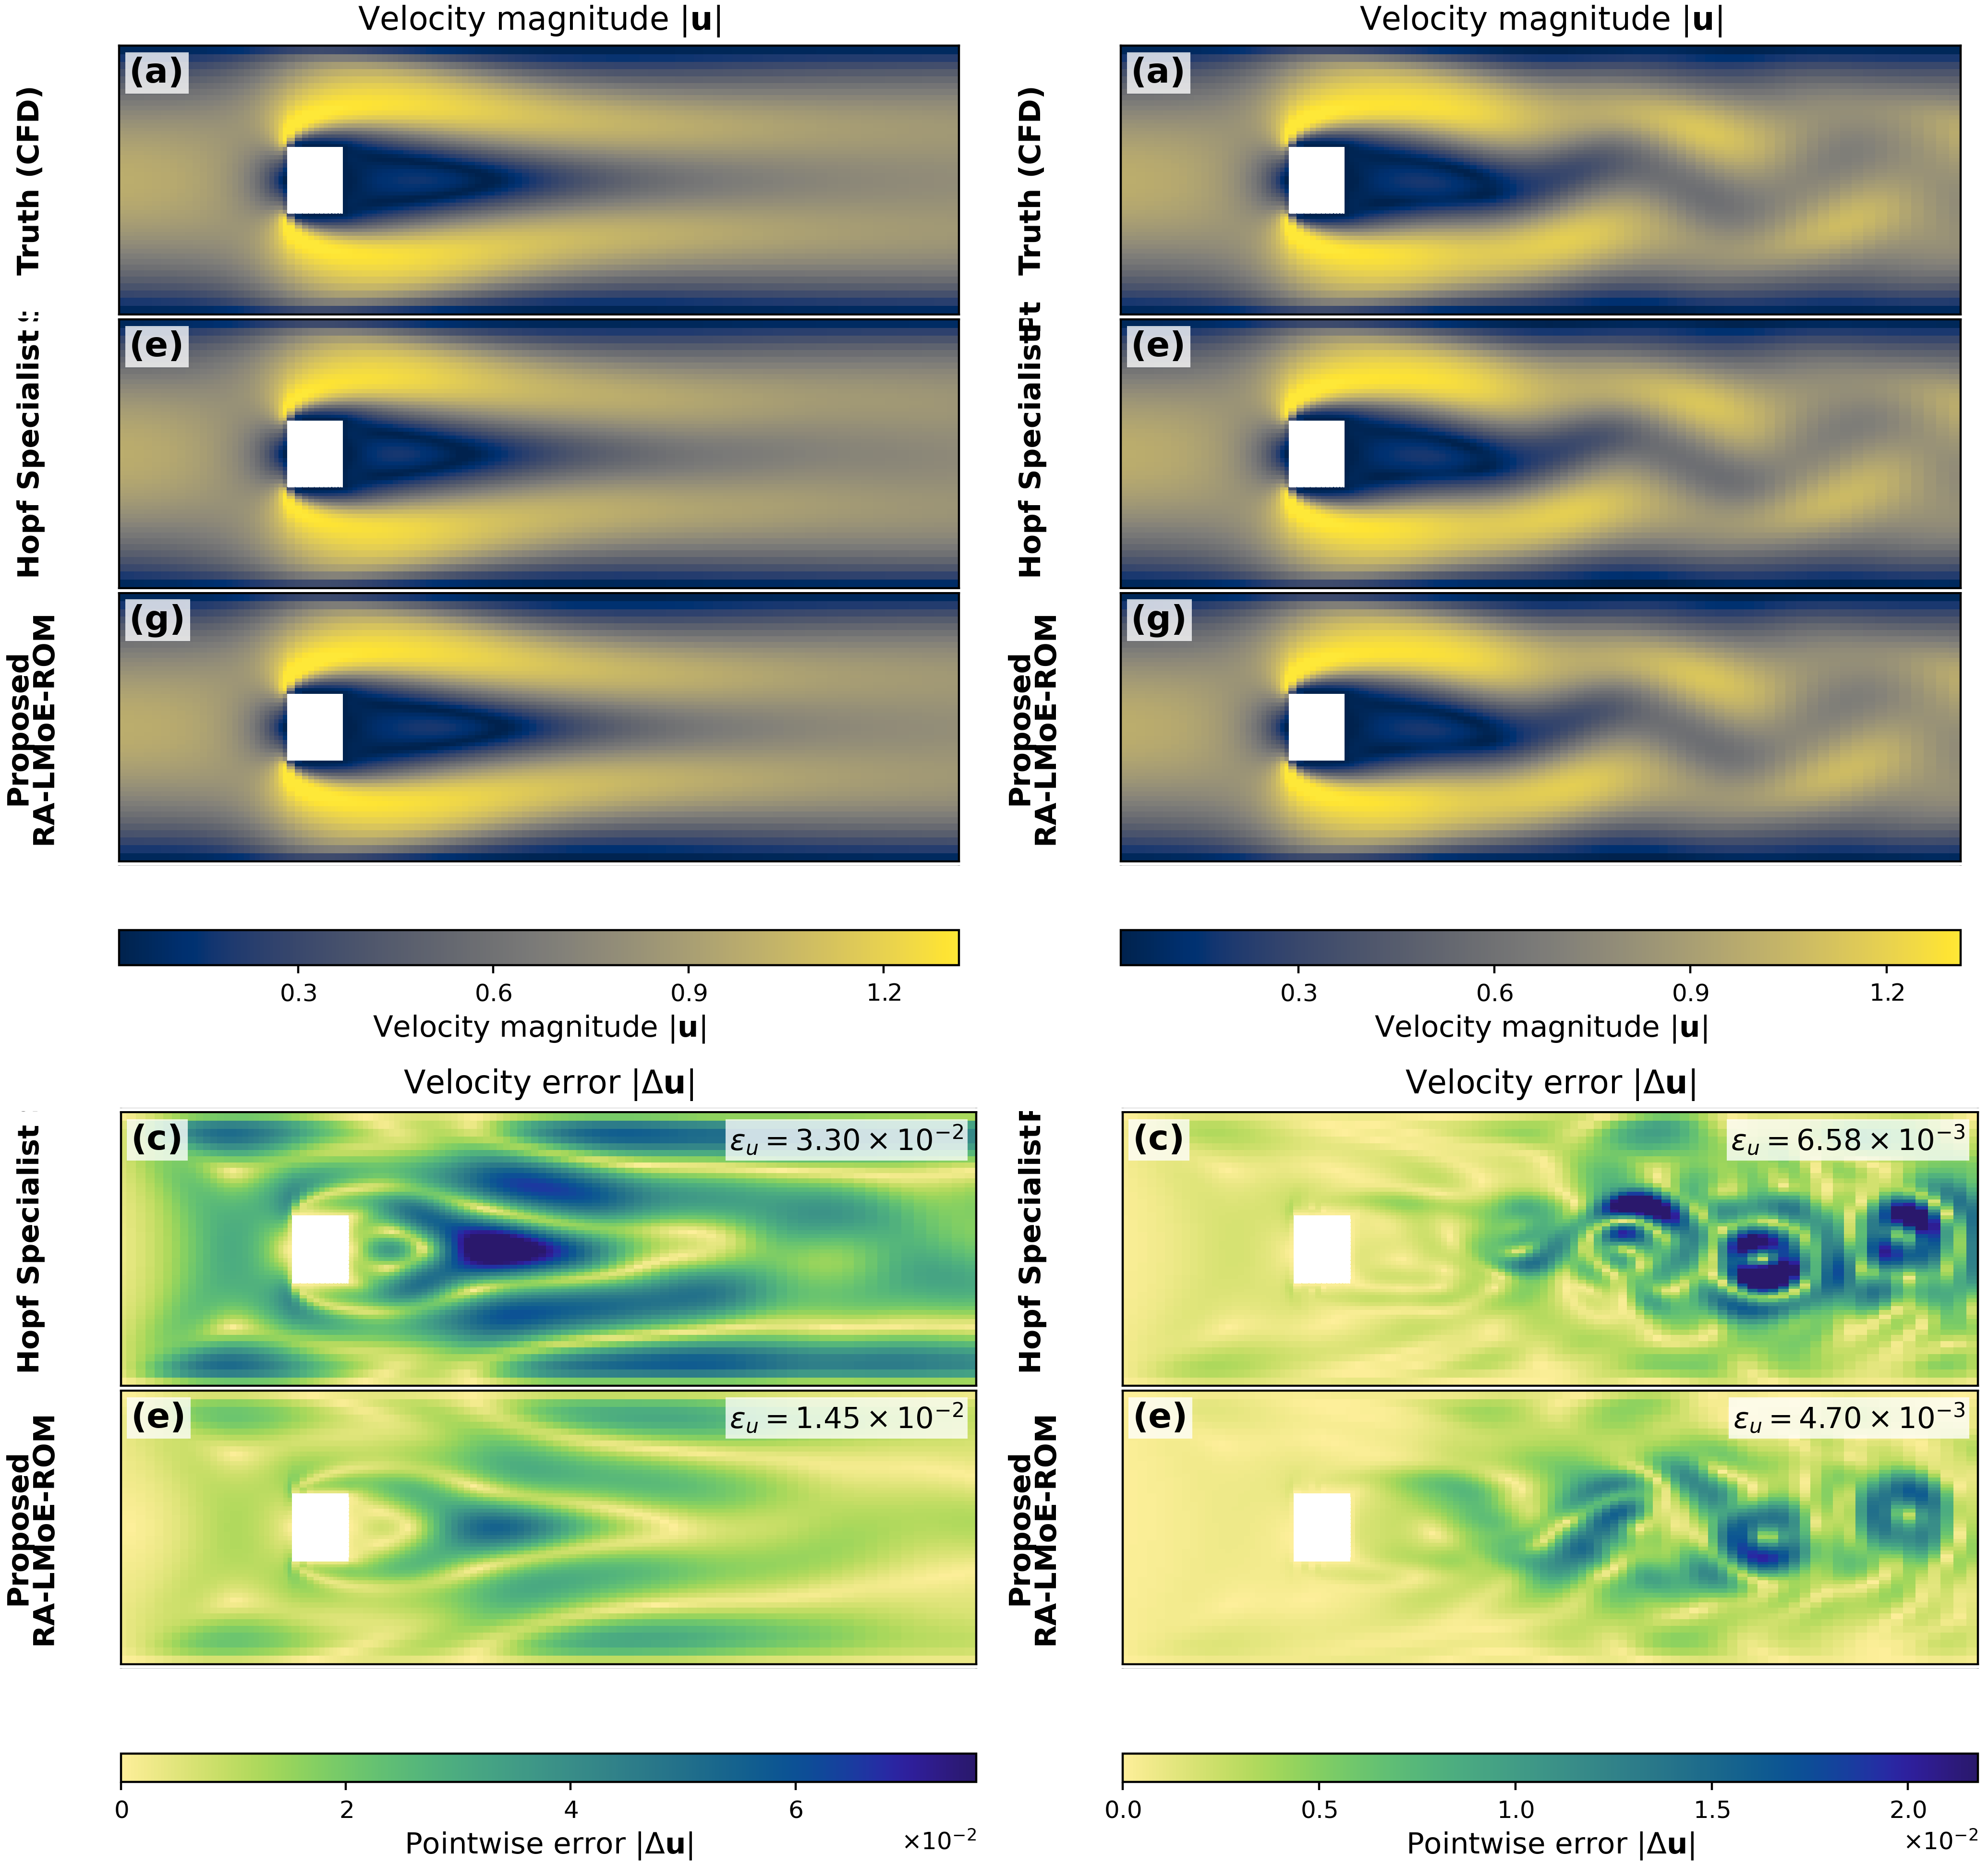
\includegraphics[width=\linewidth]{figures/square_overlap_compact.png}
\caption{Representative centered-square overlap predictions for $S$--$H$ (left) and $H$--$P$ (right). T2-C combines independently evolved local predictions only after reconstruction in physical space. The displayed examples illustrate the corresponding reduction in velocity-field error; complete velocity and pressure comparisons are reported in Appendix~\ref{app:square}.
}
\label{fig:square_overlap}
\end{figure}



\subsection{How do local architectural choices affect prediction?}

The circular-cylinder benchmark is used to examine three local architectural choices: structured expert parameterization, the projected ROM backbone, and regime localization (Table~\ref{tab:compact_ablation}). Vanilla-FNN-MoE retains the regime-local setting but replaces the structured expert map with conventional feed-forward experts. DataOnly-MoE removes the projected Galerkin and Pressure--Poisson backbone, leaving the learned local dynamics to account for the evolution from data. Global MoE replaces the regime-local charts and specialists with a single global reduced representation and dynamical model. All comparisons are reported in physical-field error so that models with different reduced coordinates are assessed in a common physical space. These comparisons characterize architectural effects under the available fixed models rather than parameter-matched capacity controls. Total and active trainable parameter counts for the analyzed Hopf and Periodic specialists are reported in Appendix~\ref{app:parameter_counts}.
\begin{table}[!htbp]
\centering
\caption{
Local architecture comparison on the circular-cylinder benchmark. Each regime cell reports the mean held-out physical-field error across
Reynolds-number trajectories, with $E_u$ on the first line and $E_p$ on the second, in percent; lower is better. N/E denotes that the Hopf Vanilla-FNN-MoE model does not satisfy the predefined validation-stage rollout criterion; no held-out result is therefore reported.
}
\label{tab:compact_ablation}
\small
\setlength{\tabcolsep}{4pt}
\begin{tabular}{@{}lccc@{}}
\toprule
Model & Steady ($K=56$) & Hopf ($K=56$) & Periodic ($K=48$) \\
\midrule
RAL-MoE-ROM
& \shortstack{0.1027\\0.7875}
& \shortstack{0.0160\\0.1338}
& \shortstack{0.2641\\3.8213} \\
\addlinespace
Vanilla-FNN-MoE
& \shortstack{0.1690\\10.3883}
& N/E
& \shortstack{2.0615\\8.6458} \\
\addlinespace
DataOnly-MoE
& \shortstack{0.3380\\16013.2835}
& \shortstack{0.2570\\1402.4380}
& \shortstack{1.3266\\6.5350} \\
\addlinespace
Global MoE
& \shortstack{0.2125\\4.4795}
& \shortstack{0.0189\\0.1721}
& \shortstack{0.8800\\4.2731} \\
\bottomrule
\end{tabular}
\end{table}
Replacing the structured expert map with conventional feed-forward experts increases both velocity and pressure errors in the Steady and Periodic regimes; the Vanilla-FNN-MoE Hopf model is not evaluable under the prescribed rollout criterion. Removing the projected ROM backbone produces the largest degradation, with particularly large pressure errors for DataOnly-MoE in the Steady and Hopf regimes. Among the ablations, Global MoE provides the closest overall comparison and is particularly close to the full model in the Hopf regime. Nevertheless, the regime-local specialists retain lower reported physical-field errors in all three regimes. Together, these comparisons support the roles of structured expert corrections, the projected ROM backbone, and regime-local representations under the tested architectures. They are not parameter-matched capacity controls. Cross-regime assembly is evaluated separately in Table~\ref{tab:routing_fusion}. Additional post-hoc internal-routing diagnostics are reported in
Appendix~\ref{app:internal_routing}.







